\chapter{Accueil et Navigation}

    Commençons par vous présenter la page centrale de notre site: la page d'accueil, que les visiteurs voient en premier c'est pourquoi nous l'avons construite de manière épurée et fonctionnelle. 

    \medskip
    \begin{figure}[!ht]
        \centering
        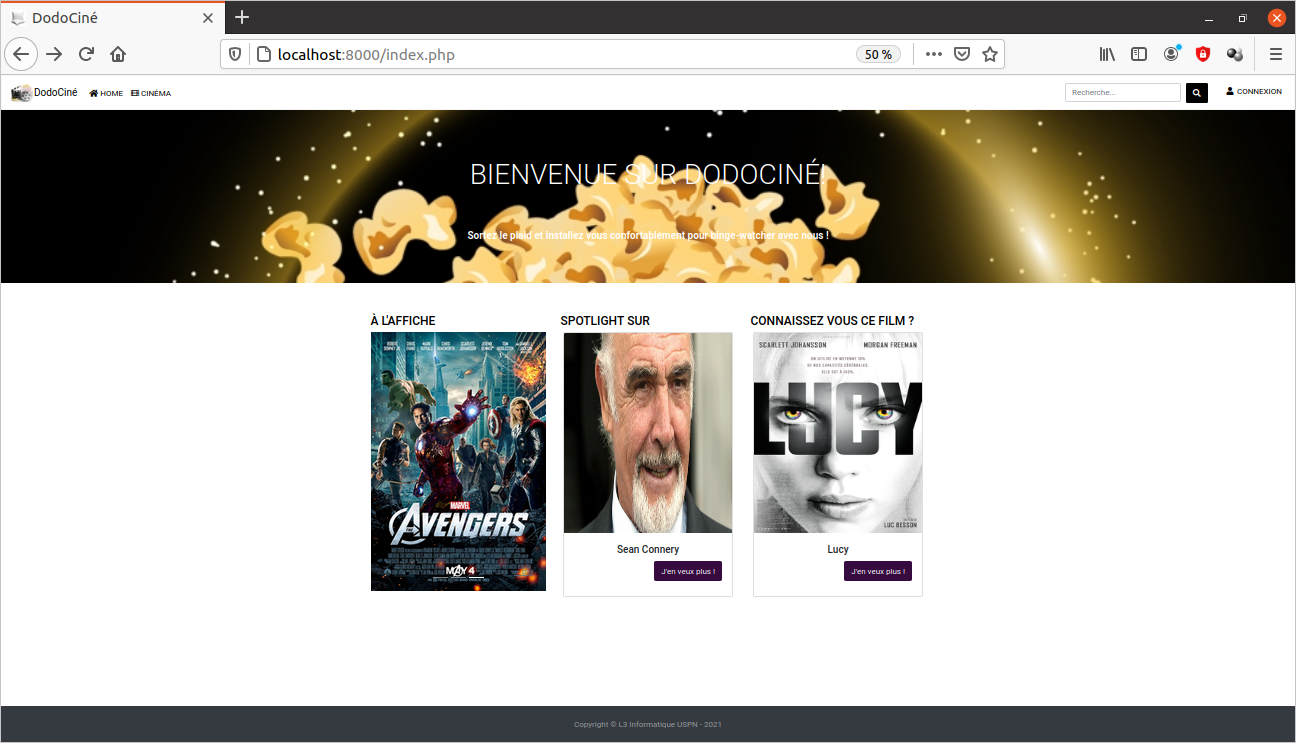
\includegraphics[width=15cm]{img/page_accueil.png}
        \caption{Page d'accueil de notre site}
    \end{figure}

    \section{Les composants de la page d'accueil}
        
        On souhaite que, dès son arrivée, le visiteur puisse avoir un aperçu des derniers films présentés sur le site. Pour ce faire, nous utilisons un "carousel", c'est-à-dire une bannière animée, pour les mettre en avant. 

        Afin de simplifier son inclusion et son interaction avec l'ensemble de la page, nous avons fait le choix d'utiliser l'élément "carousel" intégré dans le framework Bootstrap, et qui gère de façon automatique les actions dynamiques autour du "carousel".

        \medskip
        En plus de cela, nous mettons en avant un acteur/réalisateur ainsi qu'un film apparaissant de manière aléatoire avec la possibilité de visiter leur fiche pour plus d'informations.


    \section{La barre de navigation}

        Nous avons décomposé la barre de navigation en 2 parties: sur la gauche, le visiteur peut naviguer entre la page d'accueil et la liste de films disponibles sur le site (via l'onglet "Cinéma"). Sur la droite, le visiteur peut se connecter, ou s'inscrire (en créant son compte). 

        \begin{figure}[!ht]
            \centering
            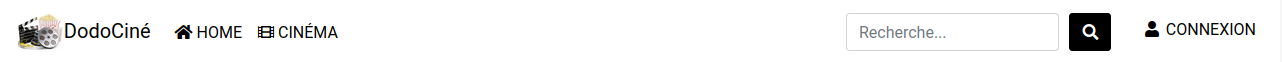
\includegraphics[width=16cm]{img/navigation.png}
            \caption{notre barre de navigation vu par un simple visiteur}
        \end{figure}

        Si le visiteur s'est connecté, alors la barre de navigation change: à la place du bouton de connexion, il voit apparaitre son pseudonyme et peut accèder à son espace personnel, ou se déconnecter.

        \begin{figure}[!ht]
            \centering
            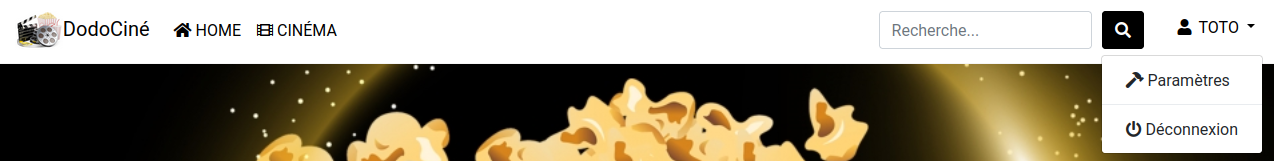
\includegraphics[width=16cm]{img/navigation-connect.png}
            \caption{notre barre de navigation lorsque le visiteur est connecté}
        \end{figure}


        \subsection{mise en place d'une recherche auto-complétée}

            \begin{figure}[!ht]
                \centering
                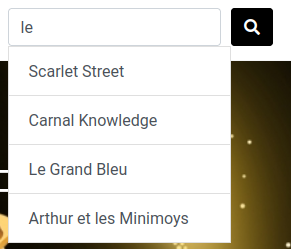
\includegraphics[scale=0.8]{img/recherche-auto.png}
                \caption{Recherche auto-complétée}
            \end{figure}

            Il est possible à tout le moment d'effectuer une recherche à propos d'un film ou d'un acteur/réalisateur en tapant son nom dans la barre de recherche du menu de navigation. Au fur et à mesure des entrées utilisateurs, nous proposons à l'utilisateur des noms de films ou d'acteurs. En cliquant sur l'un d'eux, il accède directement à la fiche du film/de l'acteur. A l'inverse, si le visiteur ne trouve pas dans les propositions ce qui lui convient, il peut simplement cliquer sur le bouton de recherche qui le renverra sur une nouvelle page contenant le résultat de sa recherche.

